\documentclass{article}
    \usepackage{pgf-umlcd, geometry, tikz, graphics, listings, float}
    \usepackage[bottom]{footmisc}

    \geometry{margin=1in}
    \usetikzlibrary{positioning, arrows.meta}

    \definecolor{whitesmoke}{rgb}{0.96, 0.96, 0.96}

    \renewcommand{\umldrawcolor}{black} %changes border colour of UML Classes
    \renewcommand{\umlfillcolor}{whitesmoke} %changes fill colour of UML Classes

    \lstset{
        language=xml,
        tabsize=3,
        %frame=lines,
        %caption=Test,
        label=code:sample,
        frame=shadowbox,
        rulesepcolor=\color{gray},
        xleftmargin=20pt,
        framexleftmargin=15pt,
        keywordstyle=\color{blue}\bf,
        commentstyle=\color{OliveGreen},
        %stringstyle=\color{red},
        numbers=left,
        numberstyle=\tiny,
        numbersep=5pt,
        breaklines=true,
        showstringspaces=false,
        basicstyle=\footnotesize,
        emph={S t r i n g L i t e r a l, PrintStatement, ElseBlock, FuncCall, Program,ReturnStatement, FuncDec,Id, FormalParam, Type, Block, VarDec, Condition,RealLiteral, IfStatement, BinExpr, IfBlock , WhileStatement, BinExpr, IntLiteral, Assign , SubExpr},emphstyle={\color{blue}}
    }

\begin{document}

\begin{titlepage}
    \begin{center}
        \vspace*{1cm}
        
        \Huge
        \textbf{CPS2002 - Software Engineering}
        
        \vspace{0.5cm} 
        \LARGE
        Course Assignment
        
        \vspace{1.5cm}
        
        \textbf{Neil Sciberras 79798M}\\
        \textbf{Franklyn Sciberras 41498M}
        
        \vfill
        
        %\vspace{0.8cm}
        
        \Large
        University of Malta\\
        Department of Computer Science\\
        21st May 2018
        
    \end{center}
\end{titlepage}

\tableofcontents
\newpage

\section{Code Coverage Analysis}
In the first section, we were to provide the code coverage metrics for the code provided for the game. The results we achieved were the following:
    
    \begin{figure}[h]
        \centering
        \includegraphics[width=\linewidth]{./Images/code_coverage_metrics.png}
        \caption{Code Coverage Metrics}
    \end{figure}

\noindent
From the previous figure we can notice that even though most of the classes have a 100$\%$ code coverage, there are some which lack the percentage, either by a small or even a large margin. In the following subsection we will explain the reasons behind such coverage.

\subsection{Metric Explanation}

\subsubsection{Game}

The first class that doesn't have a 100$\%$ code coverage metric, is the class \textbf{Game}. Such a class mainly has two methods which are not covered, as can be observed from the previous figure. These two methods are the methods:

    \begin{enumerate}
        \item \textbf{generateHTMLFiles()}
        \item \textbf{main()}
    \end{enumerate}

\noindent
The first method \textbf{generateHTMLFiles()} was not tested, since we did not feel the need to test it. Since the only job of such a method is to create a new html file for each player in the game, there was no need for software testing. In order to test that such a method is functioning properly, one only has to check the amount of players that are in game, and check the amount of html files that have been created. If they are equal, we know that the method is properly working.

\noindent
The second and final method in this class is \textbf{main()}. The main method was was not tested since it's primary function is that to prompt the user with the required output at the proper time, and gather some required information for the game to proceed. The rest of the functions it makes use of are already defined and tested for somewhere else. For such reasons there was no need to design a specific software test for such a function, since a simple run of the program would have been a necessary enough test in itself.

\subsubsection{HTMLBuilder}
The second class that doesn't have a 100$\%$ code coverage metric, is the class \textbf{HTMLBuilder}. Such a class has none of its methods covered with tests.

\noindent
The first method not to be tested is the \textbf{HTMLBuilder()}. The constructor was not tested since it's job is to create a text file with player id. In order to check whether this was working properly one could just go to the assigned file directory and check whether the file was there or not, with the proper player id's.

\noindent
The second and final method that was not tested in this class is \textbf{writeMapToFile()}. Such method was used to go to the html file produced and fill it with the appropriate code, which could correspond to the current map status. We felt no need to test such a method's functionality, since this method produced an html file which could be inspectioned physically if an error occured. If a software error, that cannot be caught by the eye occurs, such as the file could not opening, the error would be caught through exception handling.

\subsubsection{Map\_Factory}
In this class, even though all the methods were covered, we still didn't get 100$\%$ line coverage, since in the tests we only used the instance of a hazardous map. However since they both have the same architecture and only the amount of water tiles is different from the safe map, we felt no need to create another test using a safe map instance, since for these kind of tests, it would have changed nothing of any importance.

\subsubsection{Player}
\textbf{Player} is also another class, that doesn't have a 100$\%$ code coverage. This happens mainly because of two instances in the coding.

\noindent
The first instance is the instance when a random starting position is a water or treasure tile, and how would the player in terms of starting position would behave. Even though we covered such an eventuality by code, the code covering it was not tested for. This is because the map generated is randomly generated, and we have no means of knowing beforehand where these tiles will be placed. For such reasons we could not create a possible test scenario for this. However through physical testing and inspection we made sure that this part of code works fine.

\noindent
The second instance is the test regarding the \textbf{getMap()} method. This function was not tested for since it is a simple getter, which is only used to return the private map copy of the player. 

\subsubsection{Position}
Finally the final class which was not fully covered by unit testing is the class \textbf{Position}. This class only has one method which is not covered, and that is the \textbf{toString()} method. Such a method was not tested sinc it's job is to print position co-ordinates on the console. Since this method only produces an output without any other hidden logic, there was no need for testing, since any error could be easily caught visually (apart from the fact that it's use is so basic, that there is no need to test it).

\section{Design of Basic Version}

Class \textbf{Game} containing the \textbf{main method}, initially asks the user to enter the 
number of players and the size of the map. \textbf{Map}'s \textbf{setMapSize()} will return
true if the entered size and number are valid, and if not the user will keep being asked 
until he enters valid configuration details. \\

\noindent
Once the game details have been entered correctly, \textbf{startGame()} is invoked which 
sets the map size, creates the array of requested number of players, and generates a random 
initial position for each of them. An \textbf{HTMLBuilder} object is created and in turn 
generates the HTML file for each player in the game. There only exists one map in the game, 
but each player will have a different HTML file, which reveals different parts of the map 
based on where the player is. \\

\noindent
The game will then loop until the game is declared won. At each iteration, the users are 
prompted one by one to enter their next move. \textbf{Player}'s \textbf{move()} will return
true when the move was a valid one and false when not. The user will be notified when his 
move was invalid, but he is not prompted to enter a new one. \\

\noindent
When the player makes a valid move, it is checked whether the move resulted in the particular 
player stepping on the treasure or on a water tile. When moving on a water tile the player is 
moved back to his initial position using \textbf{moveToInitial}, and when he reaches the 
treasure, the corresponding flag in \textbf{Game}'s \textbf{treasureFlags[]} is set to true. 
The HTML files are updated uncovering the new tiles the player moved to. Then the 
\textbf{treasureFlags} array is iterated once to check if any player has won the game, 
and if so displays the winning message and exits the loop. \\

\noindent
The classes used and their design can be seen in \textbf{figure~\ref{fig:classes}}.

\begin{figure}[ht] %fixes the position of the figure to this point
    \centering
    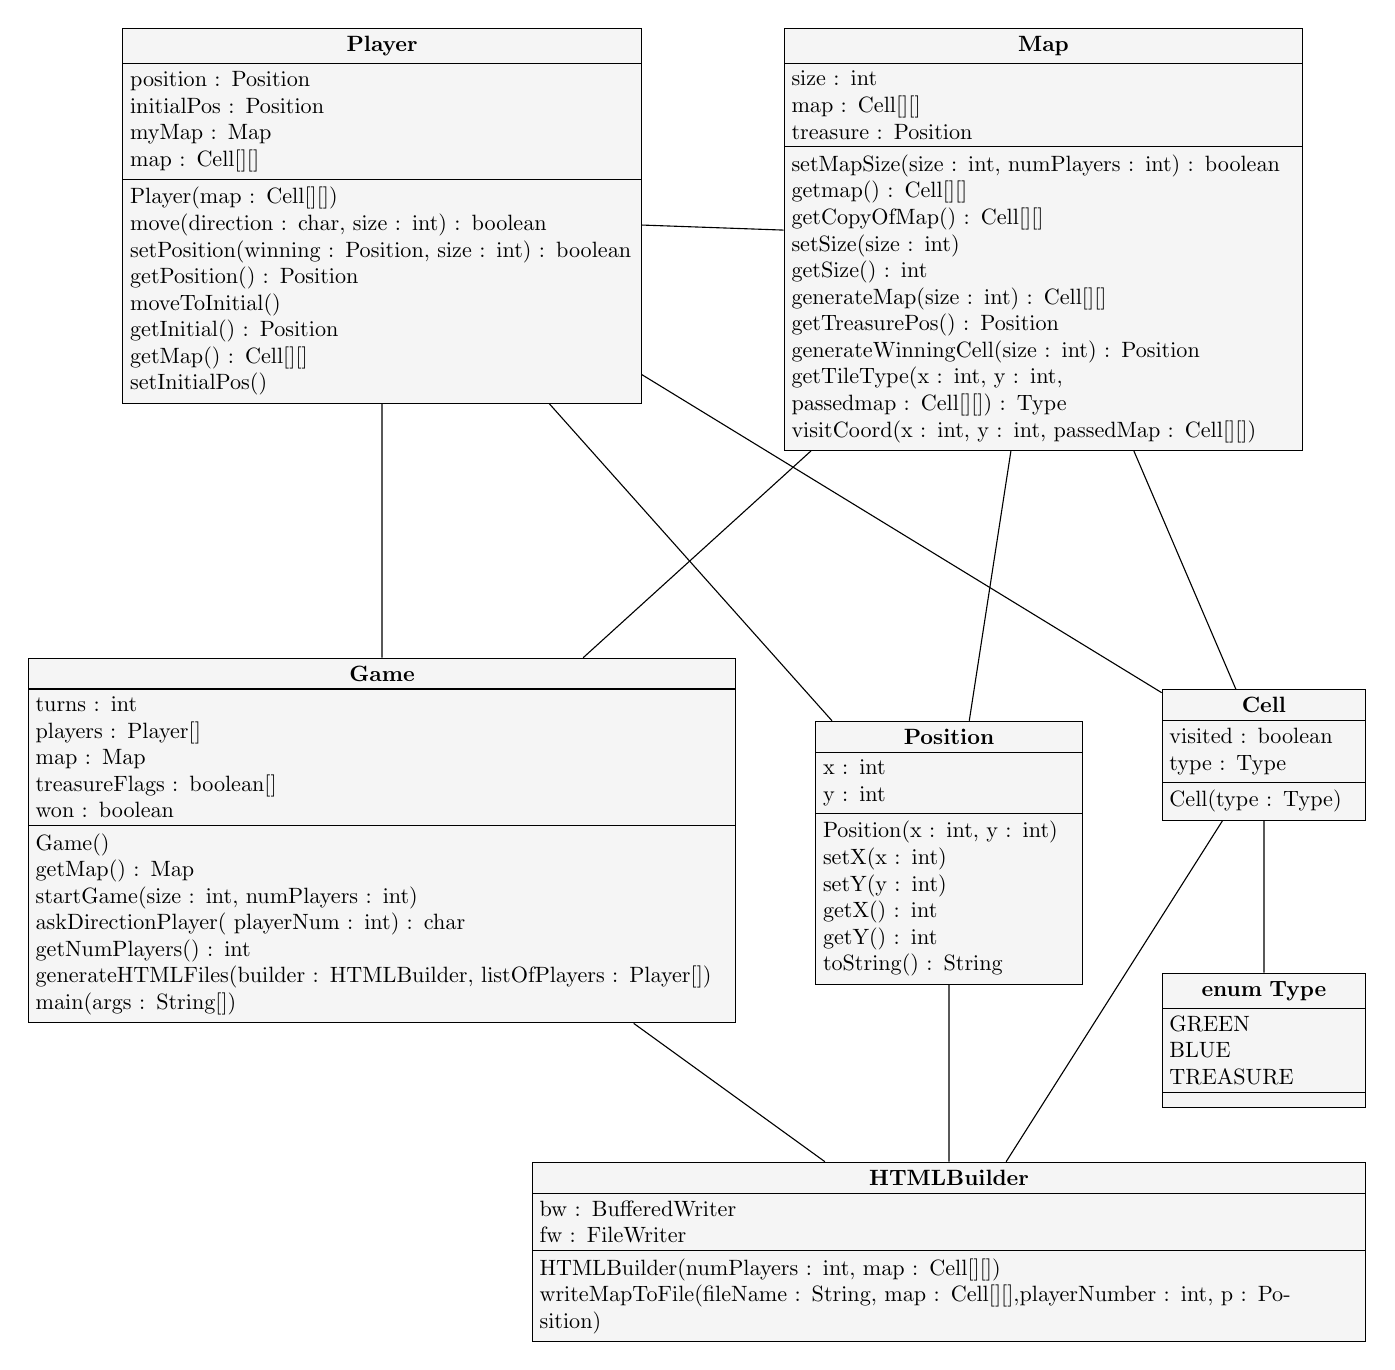
\begin{tikzpicture}[scale=0.8, every node/.style={scale=0.8}]
        
        \begin{class}[text width=11cm]{Game}{-7,-10} 
            \attribute{turns : int}
            \attribute{players : Player[]}
            \attribute{map : Map}
            \attribute{treasureFlags : boolean[]}
            \attribute{won : boolean} 

            \operation{Game()}
            \operation{getMap() : Map}
            \operation{startGame(size : int, numPlayers : int)}
            \operation{askDirectionPlayer( playerNum : int) : char}
            \operation{getNumPlayers()  : int}
            \operation{generateHTMLFiles(builder : HTMLBuilder, listOfPlayers : Player[])}
            \operation{main(args : String[])}
        \end{class}

        \begin{class}[text width=8cm]{Player}{-7,0} 
            \attribute{position : Position}
            \attribute{initialPos : Position}
            \attribute{myMap : Map}
            \attribute{map : Cell[][]}

            \operation{Player(map : Cell[][])}
            \operation{move(direction : char, size : int) : boolean}
            \operation{setPosition(winning : Position, size : int) : boolean}
            \operation{getPosition() : Position}
            \operation{moveToInitial()}
            \operation{getInitial() : Position}
            \operation{getMap() : Cell[][]}
            \operation{setInitialPos()}
        \end{class}

        \begin{class}[text width=8cm]{Map}{3.5,0} 
            \attribute{size : int}
            \attribute{map : Cell[][]}
            \attribute{treasure : Position}

            \operation{setMapSize(size : int, numPlayers : int) : boolean}
            \operation{getmap() : Cell[][]}
            \operation{getCopyOfMap() : Cell[][]}
            \operation{setSize(size : int)}
            \operation{getSize() : int}
            \operation{generateMap(size : int) : Cell[][]}
            \operation{getTreasurePos() : Position}
            \operation{generateWinningCell(size : int) : Position}
            \operation{getTileType(x : int, y : int, passedmap : Cell[][]) : Type}
            \operation{visitCoord(x : int, y : int, passedMap : Cell[][])}
        \end{class}

        \begin{class}[text width=13cm]{HTMLBuilder}{2,-18} 
            \attribute{bw : BufferedWriter}
            \attribute{fw : FileWriter}

            \operation{HTMLBuilder(numPlayers : int, map : Cell[][])}
            \operation{writeMapToFile(fileName : String, map : Cell[][],playerNumber : int, p : Position)}
        \end{class}

        \begin{class}[text width=4cm]{Position}{2,-11} 
            \attribute{x : int}
            \attribute{y : int}

            \operation{Position(x : int, y : int)}
            \operation{setX(x : int)}
            \operation{setY(y : int)}
            \operation{getX() : int}
            \operation{getY() : int}
            \operation{toString() : String}
        \end{class}

        \begin{class}[text width=3cm]{Cell}{7,-10.5} 
            \attribute{visited : boolean} 
            \attribute{type : Type}

            \operation{Cell(type : Type)}
        \end{class}

        \begin{class}[text width=3cm]{enum Type}{7,-15} 
            \attribute{GREEN}
            \attribute{BLUE}
            \attribute{TREASURE}
        \end{class}

        \association{Game}{}{}{Player}{}{}
        \association{Game}{}{}{Map}{}{}
        \association{Game}{}{}{HTMLBuilder}{}{}

        \association{Player}{}{}{Position}{}{}
        \association{Player}{}{}{Cell}{}{}
        \association{Player}{}{}{Map}{}{}

        \association{enum Type}{}{}{Cell}{}{}

        \association{Map}{}{}{Cell}{}{}
        \association{Map}{}{}{Position}{}{}

        \association{Position}{}{}{HTMLBuilder}{}{}

        \association{HTMLBuilder}{}{}{Cell}{}{}

    \end{tikzpicture}
    \caption{UML Class Diagram of the basic version of the game}
    \label{fig:classes}
\end{figure}

\newpage

\section{Enhancements}
\subsection{Different Map Types}

The \textbf{Factory Design Pattern} is used for the problem of having multiple types of maps,
and possibly more map types created in the future. This design pattern shifts the responsibility
of creating the map, from the \textbf{Game} class to a newly created \textbf{Map\_Factory} class. 
This does all the checking of which map should be created, and in turn returns the correct map
instance. It makes it possible to add more map types by simply amending the factory class, and 
leave the \textbf{Game} intact. In order to test this, two different map types, were introduced. The first map is a safe map, where only 10$\%$ of the tiles are marked as water tiles. The second kind of map is the hazardous map. This map will have between 25$\%$ and 35$\%$ of it's tiles marked as water tiles.\\

\noindent
\textbf{Game} will hold an instance of a \textbf{Map\_Factory} object, which will be used to call
its \textbf{getMap()} method. This method will in turn do the necessary checks to identify the 
type of map that is to be created and then call the constructor of \textbf{Map}, seen in 
\textbf{Listing~\ref{lst:MapConstructor}}.

\begin{figure}[ht] %fixes the position of the figure to this point
    \centering
    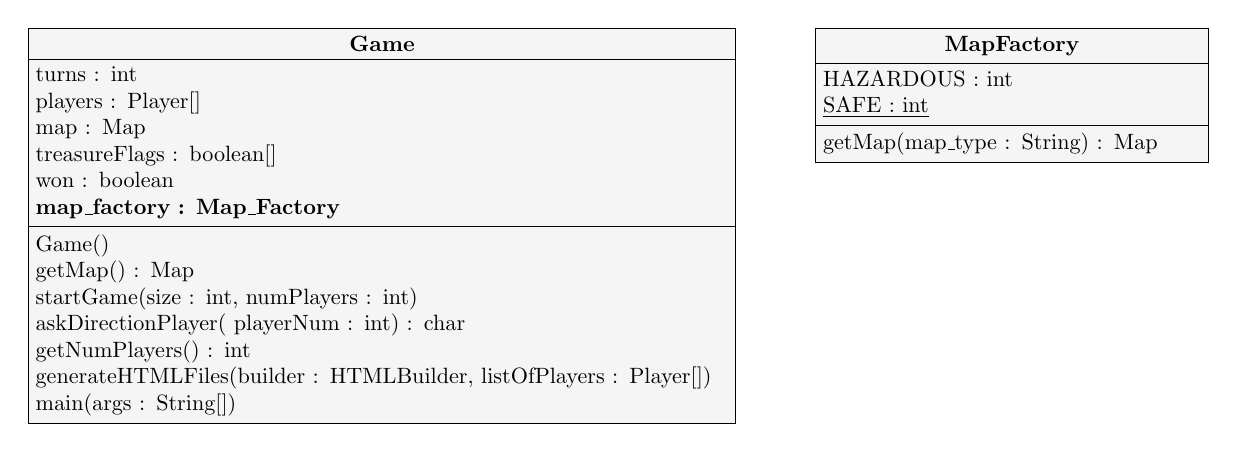
\begin{tikzpicture}[scale=0.8, every node/.style={scale=0.8}]

        \begin{class}[text width=11cm]{Game}{-12,-7} 
            \attribute{turns : int}
            \attribute{players : Player[]}
            \attribute{map : Map}
            \attribute{treasureFlags : boolean[]}
            \attribute{won : boolean} 
            \attribute{\textbf{map\_factory : Map\_Factory}}
            
            \operation{Game()}
            \operation{getMap() : Map}
            \operation{startGame(size : int, numPlayers : int)}
            \operation{askDirectionPlayer( playerNum : int) : char}
            \operation{getNumPlayers()  : int}
            \operation{generateHTMLFiles(builder : HTMLBuilder, listOfPlayers : Player[])}
            \operation{main(args : String[])}
        \end{class}

        \begin{class}[text width=6cm]{MapFactory}{-2,-7} 
            \attribute{{HAZARDOUS : int}}
            \attribute{\underline{SAFE : int}}

            \operation{getMap(map\_type : String) : Map}
        \end{class}

    \end{tikzpicture}
    \caption[caption LOF]{Factory Design Pattern UML Class Diagram\protect\footnotemark}
    \label{fig:Factory}
\end{figure}
\footnotetext{Static attributes are denoted by underline, final attributes are denoted by uppercase naming, and newly added attributes or operations are denoted by bold text}

\begin{lstlisting}[language=Java, frame=single, label={lst:MapConstructor}, caption={Constructor of class Map}, captionpos=b] 
public Map(int probability_water)
{
    this.probability_water = probability_water;
}
\end{lstlisting}

\subsection{Storing One Map in Memory}

To ensure that a single map is stored in memory, rather than one for every player, the 
\textbf{Singleton Design Pattern} is employed here. This only lets one instance of a class 
be created, and normally sets the constructor as \textbf{private} so it cannot be called.
But it was decided that all the constructor does is it sets the \textbf{probability\_water}
field of the map instance to the argument passed.\\

\noindent
When \textbf{getMapInstance()} does, is it returns the instance of the map if there is one,
and if there is no instance yet, it creates one using the constructor mentioned above. Then if 
there is the need to remove the only instance of map there is, \textbf{resetInstance()} can be called 
which just sets the instance to NULL. Having these two basic methods, now every other class that 
needs a map instance, can only call \textbf{getMapInstance()} and not the constructor. 

\begin{figure}[H] %fixes the position of the figure to this point
    \centering
    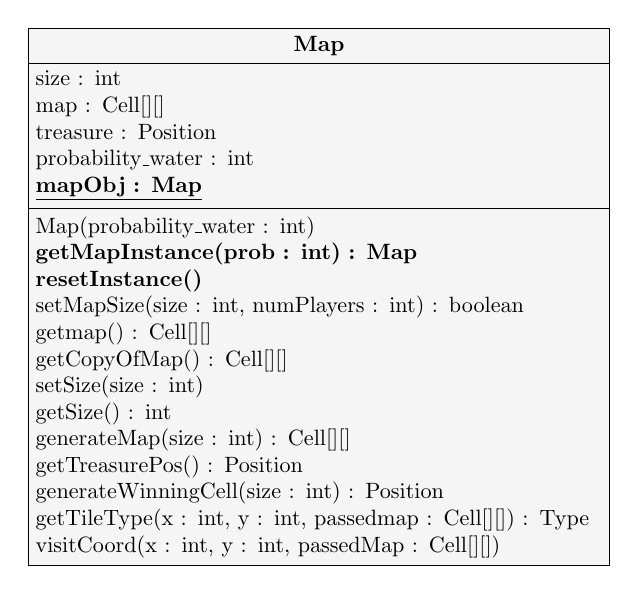
\begin{tikzpicture}[scale=0.8, every node/.style={scale=0.8}]

        \begin{class}[text width=9cm]{Map}{3.5,0} 
            \attribute{size : int}
            \attribute{map : Cell[][]}
            \attribute{treasure : Position}
            \attribute{probability\_water : int}
            \attribute{\textbf{\underline{mapObj : Map}}}

            \operation{Map(probability\_water : int)}
            \operation{\textbf{getMapInstance(prob : int) : Map}}
            \operation{\textbf{resetInstance()}}
            \operation{setMapSize(size : int, numPlayers : int) : boolean}
            \operation{getmap() : Cell[][]}
            \operation{getCopyOfMap() : Cell[][]}
            \operation{setSize(size : int)}
            \operation{getSize() : int}
            \operation{generateMap(size : int) : Cell[][]}
            \operation{getTreasurePos() : Position}
            \operation{generateWinningCell(size : int) : Position}
            \operation{getTileType(x : int, y : int, passedmap : Cell[][]) : Type}
            \operation{visitCoord(x : int, y : int, passedMap : Cell[][])}
        \end{class}        

    \end{tikzpicture}
    \caption{Singleton Design Pattern UML Class Diagram}
    \label{fig:Singleton}
\end{figure}

\subsection{Team Exploration}

When teams are introduced into the game, players need to be able to see every tile that 
members in their team have visited. This means that the HTML files of players need to be 
amended, whenever there is a change in any of the members' files. This can be implemented 
by having a central HTML file for each team, and each member is required to update this 
central HTML file apart from updating his own. Then all the members' files are registered 
as observers of this central file so that they can be updated automatically. Note that this enhancement was not finished in time due to time restrictions. In the source code one can only find it's first version class \textbf{flagWatcher}. This class would be watching the array which holds who has won and who has not, and whenever a player from a team has won, it would notify all of the observers of the players of the same team that they have won. 

\section{Screenshots}

\subsection{Initialisation Of Different Maps}

\noindent
As previously mentioned, there are currently two kind of maps implemented in the game. Below we will see an unveiled map, one of each kind. From these figures, one can notice that \textbf{Map\_Factory} class is working as designed, since we are able to see a difference in the instance of the map created, depending on the type of map. 

	\begin{figure}[h]
		\centering
	    \includegraphics[width=0.6\linewidth]{./Images/safe_map.png}
		\caption{Safe Map}
	\end{figure}

    \begin{figure}[h]
        \centering
        \includegraphics[width=0.6\linewidth]{./Images/hazardous_map.png}
        \caption{Hazardous Map}
    \end{figure}

\clearpage


\subsection{Player Stepping On Water Tile}

\noindent
From the given game description, we know that whenever a player steps on a water tile, he should be put back on his starting tile. In the following figure we can see that the player performed two left moves, however on his second left move he found himself upon a water tile. In that instance the game notified the player of the occurence and put him back on his initial tile.

    
    \begin{figure}[h]
        \centering
        \includegraphics[width=0.7\linewidth]{./Images/player_1_lose_map.png}
        \caption{Map Instance - Step On Water}
    \end{figure}

    \begin{figure}[h]
        \centering
        \includegraphics[width=\linewidth]{./Images/player_1_lose.png}
        \caption{Game Output - Step On Water}
    \end{figure}

\clearpage

\subsection{Player Winning}

\noindent
In order for the game to finish, at least one player has to find the treasure. If multiple players find the treasure in the same round, they all win. In the following case scenario, player 0 was the only player to find the treasure. The game got hold of that instance, and notified the player accordingly as we can see from the following two figures.

    \begin{figure}[h]
        \centering
        \includegraphics[width=0.7\linewidth]{./Images/player_0_win_map.png}
        \caption{Map Instance - Find Treasure}
    \end{figure}

    \begin{figure}[h]
        \centering
        \includegraphics[width=0.6\linewidth]{./Images/player_0_win.png}
        \caption{Game Output - Find Treasure}
    \end{figure}

\footnotetext{Note that the previous screenshots were captured from different games.}

\clearpage

\section{Instructions}
In order to run and play the game, the following steps have to be taken:

    \begin{enumerate}
        \item Open the game project in IntelliJ
        \item Build the project locally
        \item Run the main class Game.java
        \item The terminal will ask you to enter an amount of players. You should be able to enter between 2 to 8 players. If these numbers are not respected you will be notified accordingly.
        \item Enter the map size you and your partner/s wish to be playing in. If you are between 2 and 4 players, the minimum map size you can choose will be that of 5 by 5. If you are between 5 and 8 players the minimum map size you can choose will be that of 8 by 8. The maximum map size will be that of 50 by 50 at all times. If these numbers are not respected you will be notified accordingly.
        \item You are to choose between a safe version of the map or a hazardous version of the map, by pressing 1 or 2 respectively. Any other input will be assumed as the default map, i.e. the safe map. 
        \item Now an html file for each player will be generated in the directory where there is the project file. Each player is to open his html file, which is denoted by the player number. 
        \item The game will prompt each player to input a direction he wants to move in. You are to input one direction choosing from r:right, l:left, u:up and d:down.
        \item After all the players have input their choice, they will be prompted with their new position, or if any special occurence, happened (ex. player/s won or player/s stepped on a water tile), they will be notified.
        \item After all the players have read their notification from the terminal, each player is to press refresh on the browser holding his html file to see his current position on the map.
        \item You are to go back to step 8, up untill there is a winner.
    \end{enumerate}



\end{document} 